\chapter{Hyper-Parameters selection and babysitting}

\section*{Sanity test}
Make sure that you can overfit very small portion of the training data. Take ~20 samples, turn off regularization and make sure that you can get a loss of ~0. If you can't overfit there is a problem: or there is something broken or you have to scale up your network.

\section*{Learning Rate}
Start with small regularization (0.00001) and find learning rate that makes the loss not go down.  Then, find learning rate that makes the loss go down but at some point it explodes. The learning rate is in between this range.
\begin{figure}[h]
  \centering
  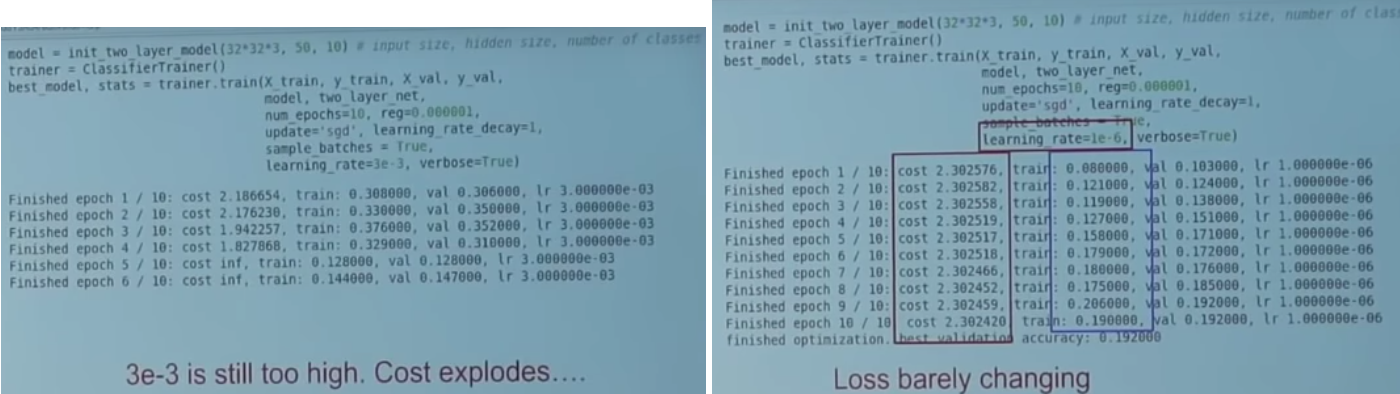
\includegraphics[width=\textwidth]{Images/hyper_params_tun/9.png}
  \caption{\textbf{Left}: Loss exploding, \textbf{Right}: Loss not going down}
\end{figure}
\begin{itemize}
\item Loss not going down: learning rate too low. Something funny can happen in this case. Loss not going down but accuracy improving until ~20\%. How is that possible? So because of the way softmax is computed, small changes in the lost can cause small changes in the scores which make the correct class has a tiny bigger score than the others. This, makes the softmax classifier get more samples correct.
\item Loss exploding (NaN happens): learning rate too high
\end{itemize}



\section*{Hyperparameter Optimization - Coarse to fine serach}
Tuning regularization and learning rate. Do coarse -> fine for cross-validation in stages. In other words, first do a rough search, see what it works, and keep iterating to longer narrow in ranges that are working. First, only a few epochs to get rough idea of what parameters work (few minutes is enough). Second, longer running time, finer search.

Also, it is better to optimize parameters in log space because reg and learning rate work manipulatively in the dynamics of your back propagation.

\begin{figure}[h]
  \centering
  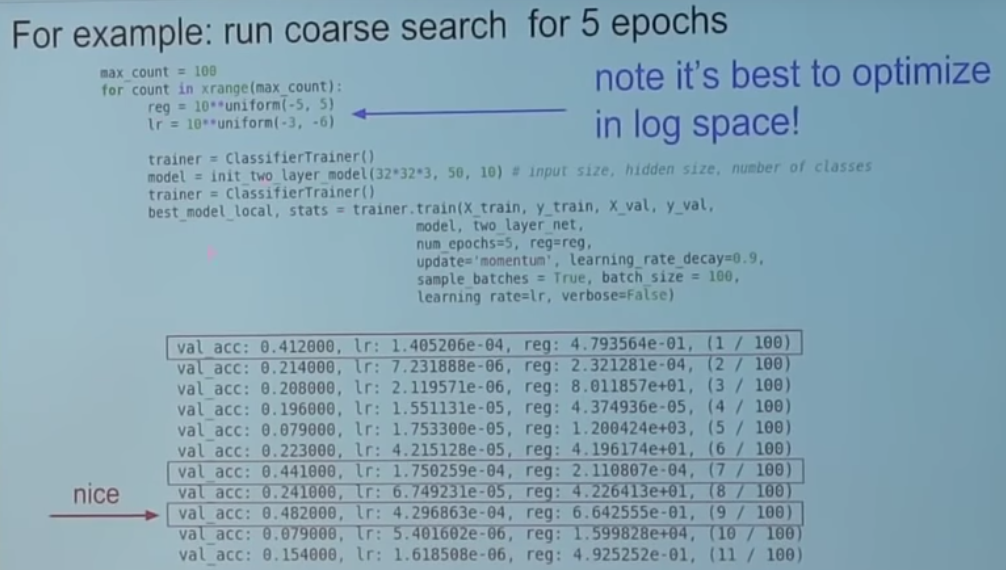
\includegraphics[width=0.6\textwidth]{Images/hyper_params_tun/3.png}
  \caption{First pass - coarse search}
\end{figure}

\begin{figure}[h]
  \centering
  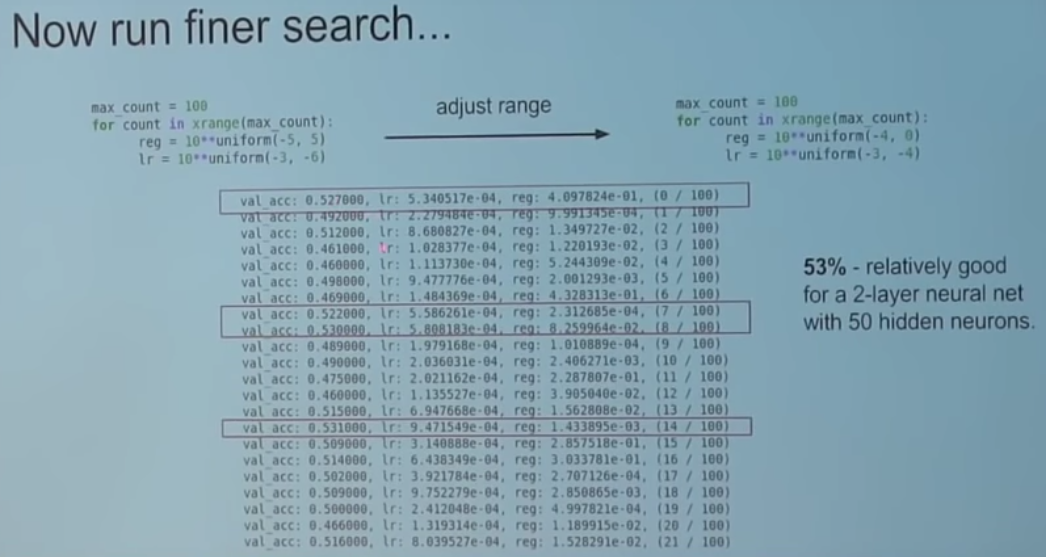
\includegraphics[width=0.6\textwidth]{Images/hyper_params_tun/4.png}
  \caption{Second pass - finer search. Notice that there is a problem with this result. The best result (last red box) has a lr close to the boundary of search that we have set (-3). So it may we better results waiting for lower values of lr. \textbf{Careful with best values on border}}
\end{figure}


\section*{Hyper-parameter Optimization - NEVER do grid (iterative) search of parameters, do random search}

\begin{figure}[h]
  \centering
  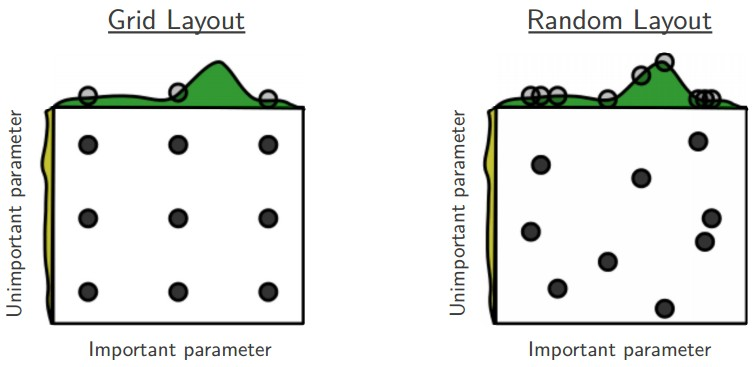
\includegraphics[width=0.5\textwidth]{Images/hyper_params_tun/5.jpeg}
  \caption{Second pass - finer search. Notice that there is a problem with this result. The best result (last red box) has a lr close to the boundary of search that we have set (-3). So it may we better results waiting for lower values of lr. \textbf{Careful with best values on border}}
\end{figure}

For cross-validation, use random search in stead of grid search. The issue is that one of the parameters may be much important than another one.

In this figure in particular its more important the x than the y dimension. Then, with random sampling, your are going to evaluate more different samples of the x parameter space (9 with random vs 3 with grid).

\section*{Hyper-parameter Optimization - Monitor and visualize the loss curve}
\begin{figure}[h]
  \centering
  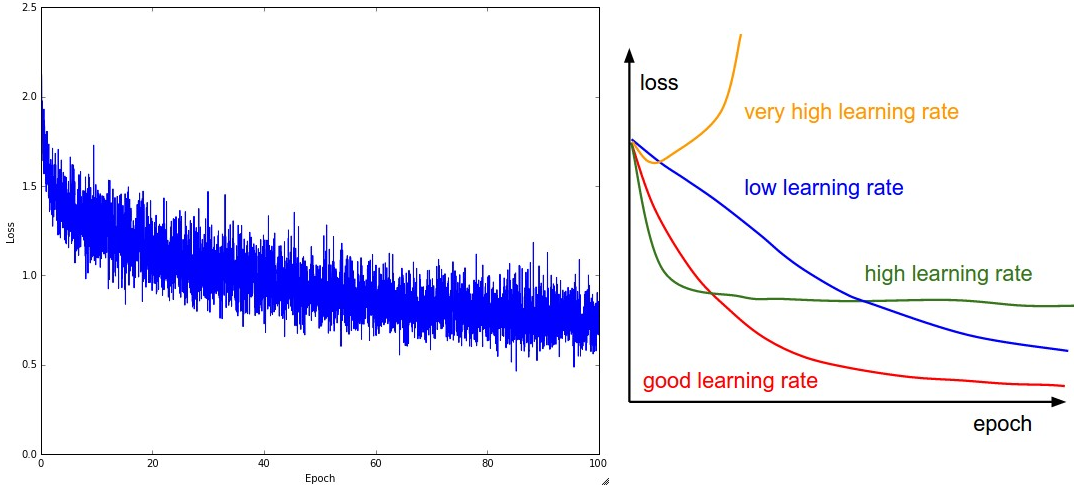
\includegraphics[width=0.65\textwidth]{Images/hyper_params_tun/10.png}
  \caption{In this left case the loss is too slow... The learning rate is too low}
\end{figure}


\section*{Hyper-parameter Optimization - Monitor and visualize the accuracy}
\begin{figure}[h]
  \centering
  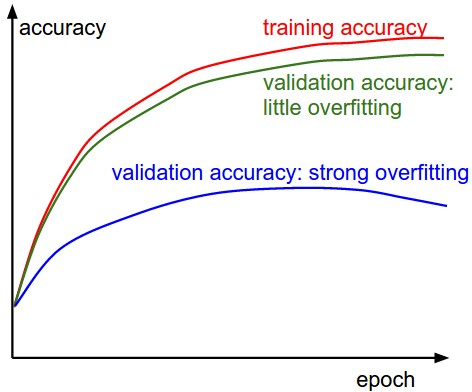
\includegraphics[width=0.3\textwidth]{Images/hyper_params_tun/8.jpeg}
  \caption{Monitor and visualize the accuracy}
\end{figure}
The gap between the training and validation accuracy indicates the amount of overfitting. Two possible cases are shown in the diagram on the left. The blue validation error curve shows very small validation accuracy compared to the training accuracy, indicating strong overfitting (note, it's possible for the validation accuracy to even start to go down after some point). When you see this in practice you probably want to increase regularization (stronger L2 weight penalty, more dropout, etc.) or collect more data. The other possible case is when the validation accuracy tracks the training accuracy fairly well. This case indicates that your model capacity is not high enough: make the model larger by increasing the number of parameters.

\begin{itemize}
\item gap between train\/val is too big: overfitting, increase regularization
\item gap between train\/val too small: increase model capacity
\end{itemize}

In this figure case there is a big gap so it is probably over-fitting. We should increase the regularization factor.

\section*{Hyper-parameter Optimization - Track the ratio of weight updates / weight magnitudes}
You want \texttt{weight\_updates / weight\_magnitudes =~0.001}.
\begin{itemize}
\item If this is too high to decrease learning rate
\item If it is too low to increase learning rate
\end{itemize}


\section*{Dropout not working}
If dropout is not working for you, you should probably be using a bigger network.